\section{Einführung}
<<<<<<< HEAD

\subsection{Aufgabenstellung}
Ziel dieser Arbeit ist es, die Uni-DB, welche auf einer SQL Server liegt, in eine NoSQL-Datenbank zu implementieren. Dazu Wird das ER-Schema der Uni-DB so umgezeichnet werden, dass es in der gewählten NoSQL-Datenbank abgebildet werden kann. Dieses Schema wird dann in der entsprechend gewählten Datenbank umgesetzt. Dazu migriert man die Daten aus der SQL- in die NoSQL-Datenbank.
Anschliessend setzt man das vorgegebene Querry (siehe Aufgabenstellung) so um, dass es in der entsprechend gewählten Datenbank benutzt werden kann. Dazu schreibt man eine Abfrage oder erstellt ein einfaches GUI.

\newpage
\subsection{Datenbankauswahl}
Bei der Auswahl der Datenbank haben wir uns für Die MongoDB entschieden. Entscheidend waren dabei folgende Gründe:
=======
Im Modul DMG wurde zu Übungszwecken zu relationalen Datenbanken die Uni-DB 
verwendet. Das dabei verwendete Entity-Relation Diagramm ist in Abbildung
\ref{fig:uni-db} ersichtlich.
\begin{figure}[htbp] 
  \centering
     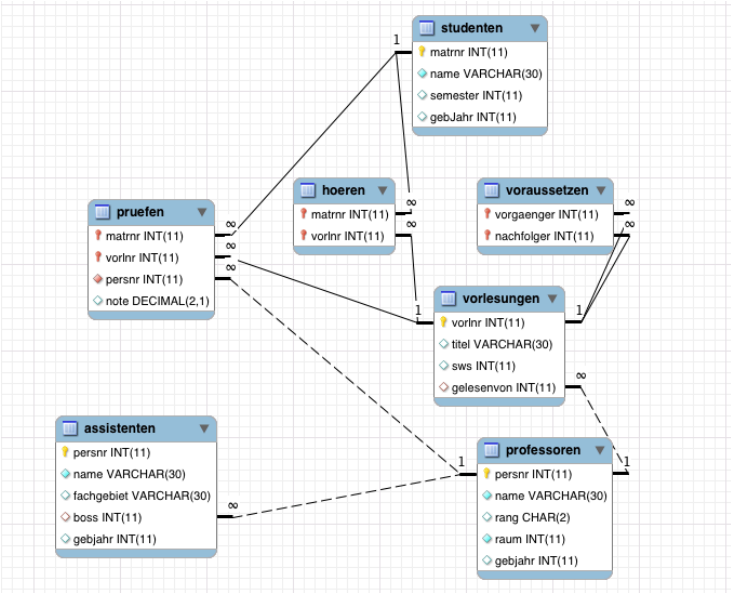
\includegraphics[width=1\textwidth]{./pictures/SQL-DB_ER_Diagramm_UNI-DB.png}
  \caption{ER-Diagramm zur Uni-DB \cite{Kaufmann2016_S1}}
  \label{fig:uni-db}
\end{figure}
 Um mit den NoSQL Datenbanken Erfahrung zu sammeln, wird dieses Schema in die NoSQL Datenbank MongoDB überführt.
Die MongoDB ist eine dokumentorientierte Datenbank und  wird aus folgenden
Gründen für dieses Projekt verwendet:
>>>>>>> 19b6044aca54f9cb01a825d558cf3a193f181206
\begin{itemize}
  \item Geeignet um unser Problem zu lösen.
  \item Wird in der Praxis eingesetzt
  \item Bekannt
  \item Gute Dokumentation
  \item Kostenlos
  \item Unterstützung durch Forenuser
  \item Erste Erfahrung vorhanden
\end{itemize}
<<<<<<< HEAD

Die MongoDB ist eine Datenbank, welche sich grundlegend im CAP Theorem in der Spalte CP aufhält. Dies bedeutet, dass die Konsitenz (Consistency) gewährleistet ist. Dies wird realisiert, indem in einem System ein Knoten als primäres Mitglied fungiert, und alle Anfragen über diesen Knoten abgearbeitet werden. Zusätzlich wird die Partition-Tolerance gewährleistet. Dies Funktioniert laut Vertreiber, indem wenn der Primäre Knoten ausfällt, automatisch ein sekundärer Knoten als neuer Primärknoten Definiert wird und somit das System wieder funktioniert.
Ebenfalls soll es möglich sein, auf Kosten der Konsistenz (Consistency) die Verfügbarkeit (Availaility) zu erhöhen, indem man in den Einstellungen die Konfiguration vornimmt, dass Daten nicht bloss über den Primär-Knoten, sondern auch über Sekundärknoten bezogen werden können.


%An die MonogDB wird eine Abfrage definiert, welche das selbe Resultat ergibt,
%wie das folgende SQL-Query:
%
%\begin{lstlisting}
%select ProfessorName, AnzahlStudenten, SummeSWS 
%from ( 
%select p.Name as ProfessorName, count(s.MatrNr) 
%as AnzahlStudenten 
%from Professoren p 
%join Vorlesungen v on v.gelesenVon = p.PersNr
%join hoeren h on h.VorlNr = v.VorlNr 
%join Studenten s on s.MatrNr = h.MatrNr 
%group by p.Name 
%) A 
%join 
%( 
%select p.Name as ProfessorName,  sum(SWS) 
%as summeSWS 
%from Professoren p 
%join Vorlesungen v on v.gelesenVon = p.PersNr 
%group by p.Name 
%) B using(ProfessorName)
%\end{lstlisting}
=======
Die Aufgabe besteht darin, ein vorgegeben SQL-Query so in MongoDB Operationen
abzubilden, dass die MonogDB Abfrage das selbe Resultat ergibt wie das folgende 
SQL-Query
\begin{lstlisting}
select ProfessorName, AnzahlStudenten, SummeSWS 
from ( 
	select p.Name as ProfessorName, count(s.MatrNr) 
	as AnzahlStudenten 
		from Professoren p 
		join Vorlesungen v on v.gelesenVon = p.PersNr
		join hoeren h on h.VorlNr = v.VorlNr 
		join Studenten s on s.MatrNr = h.MatrNr 
		group by p.Name 
	) A 
join 
( 
	select p.Name as ProfessorName,  sum(SWS) 
	as summeSWS 
	from Professoren p 
	join Vorlesungen v on v.gelesenVon = p.PersNr 
	group by p.Name 
) B using(ProfessorName)
\end{lstlisting}
>>>>>>> 19b6044aca54f9cb01a825d558cf3a193f181206
